\section{Results}

We finally implemented our RSP heuristic algorithm on a simple aircraft design problem. 
In this problem, we conduct an aerostructural optimization of a wing and fuselage given a payload and a range requirement. 

% We implemented the RSP formulation ideas above on a simple aircraft design problem, with 12 uncertain variables,
% and a single signomial constraint. . A short overview of the model follows.

\subsection{Optimization Results}

The problem is optimized for different sizes of box and elliptical uncertainty sets
by varying the parameter $\Gamma$ as defined in Appendix \ref{LP_to_GP}.
The design variables are then fixed for each solution so that the design can be simulated for
1000 different realizations of the uncertain parameters in Table~\ref{tab:uncertainties}
to examine average design performance.\\

\begin{figure}[ht]
    \centering
    \captionsetup{justification=centering, font=small}
    \begin{subfigure}{0.49\textwidth}
        \centering
        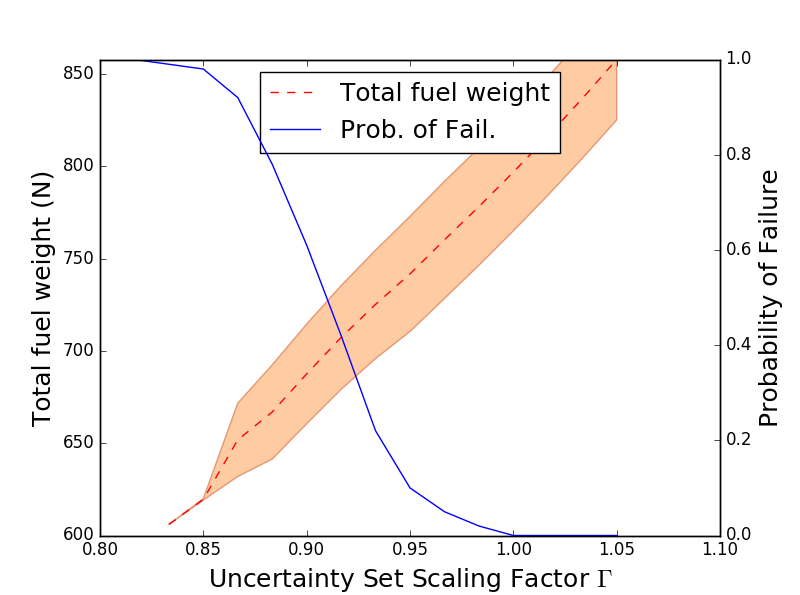
\includegraphics[height=2.3in]{signomial_simple_flight/box_best_pairs.png}
        % \caption{Box Uncertainty Set Objective Value}
    \end{subfigure}%
    ~ 
    \begin{subfigure}{0.49\textwidth}
        \centering
        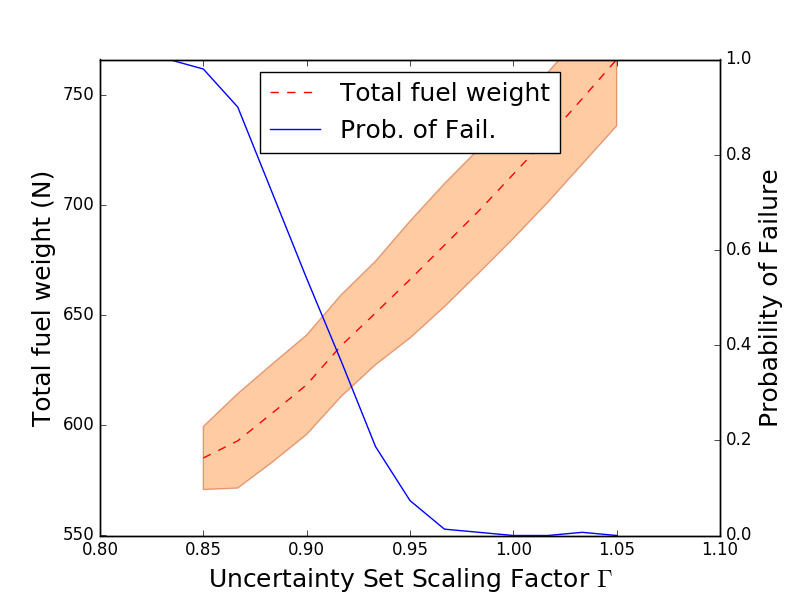
\includegraphics[height=2.3in]{signomial_simple_flight/ell_best_pairs.png}
        % \caption{Box Uncertainty Set Probability of Failure}
    \end{subfigure}
    \caption{Performance of the optimal robust signomial simple aircraft, using the Best Pairs formulation, as a function of $\Gamma$ for different uncertainty sets.}
    \label{signomial_var_gamma}
\end{figure}

We can see from Figure \ref{signomial_var_gamma} that probability of failure goes to zero as $\Gamma$ increases. 
Obviously, it is worth using elliptical uncertainty sets for this aircraft design problem as the performance is significantly better than that of a box uncertainty set, despite the increase in complexity. 
Moreover, using margins would in the best case be as good as using a box uncertaintyset, and therefore will lead to an inferior performance.

Figure~\ref{compare_signomial} compares the different methodologies in terms of run times, number of constraints, and average performance. The Best Pairs and Linearized Perturbations achieves good performance, however the Best Pairs methodology needs the most number of constraints, while the Linearized perturbations requires the most setup and solve time. The Simple Conservative formulation is significantly faster than the other formulations and requires the least number of additional constraints.
\ \\
\ \\

\begin{figure}[ht]
    \centering
    \captionsetup{justification=centering, font=small}
    \begin{subfigure}{0.499\textwidth}
        \centering
        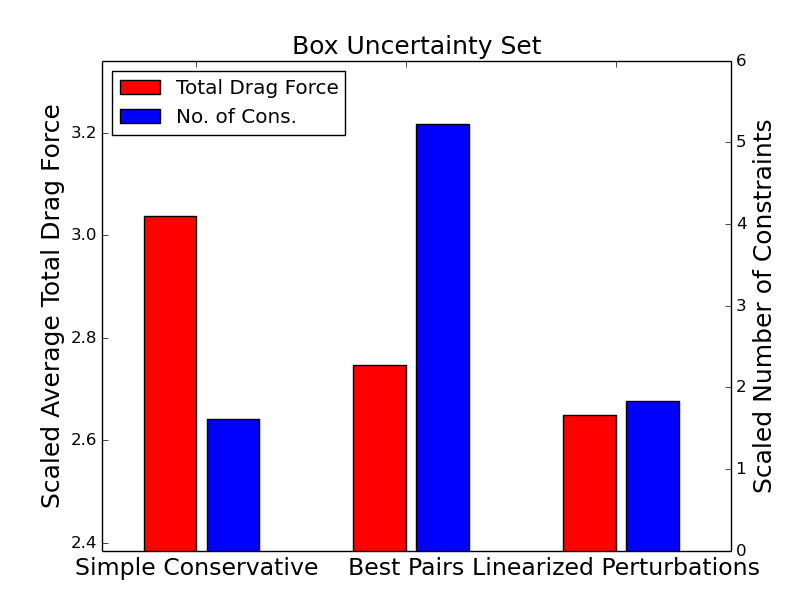
\includegraphics[height=2.3in]{signomial_simple_flight/box.png}
        % \caption{Box Uncertainty Set Objective Value}
    \end{subfigure}%
    ~ 
    \begin{subfigure}{0.49\textwidth}
        \centering
        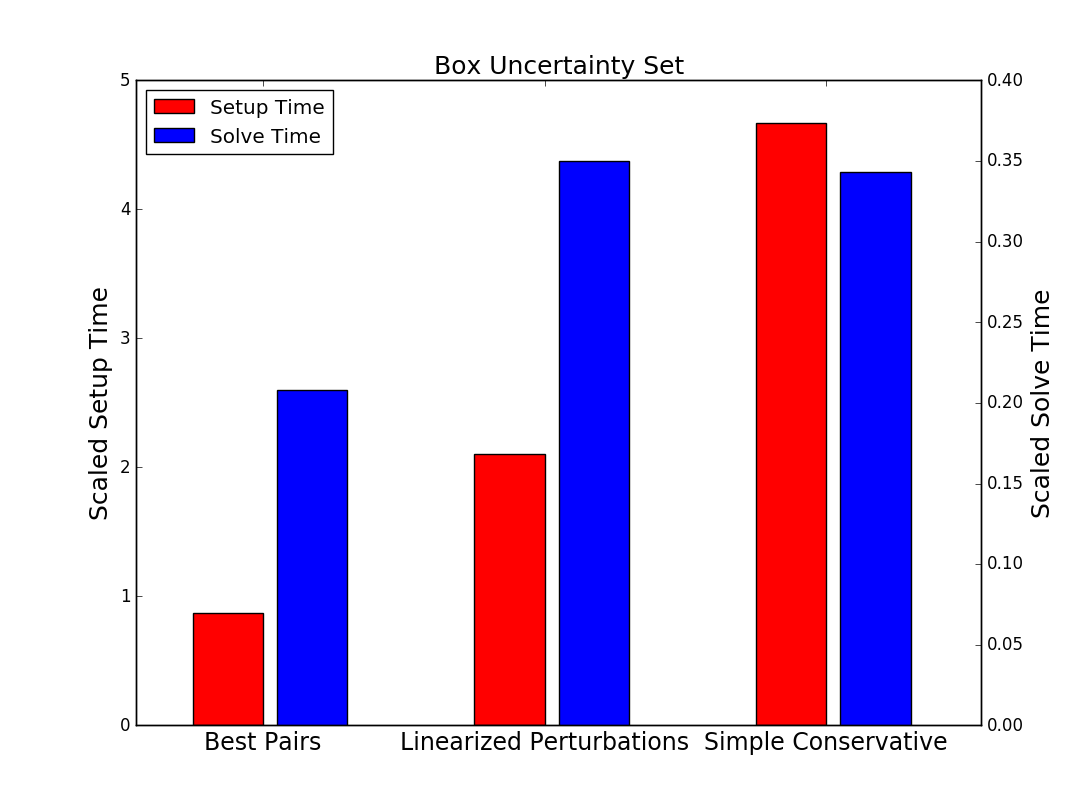
\includegraphics[height=2.3in]{signomial_simple_flight/box_times.png}
        % \caption{Box Uncertainty Set Probability of Failure}
    \end{subfigure}
    ~
    \begin{subfigure}{0.499\textwidth}
        \centering
        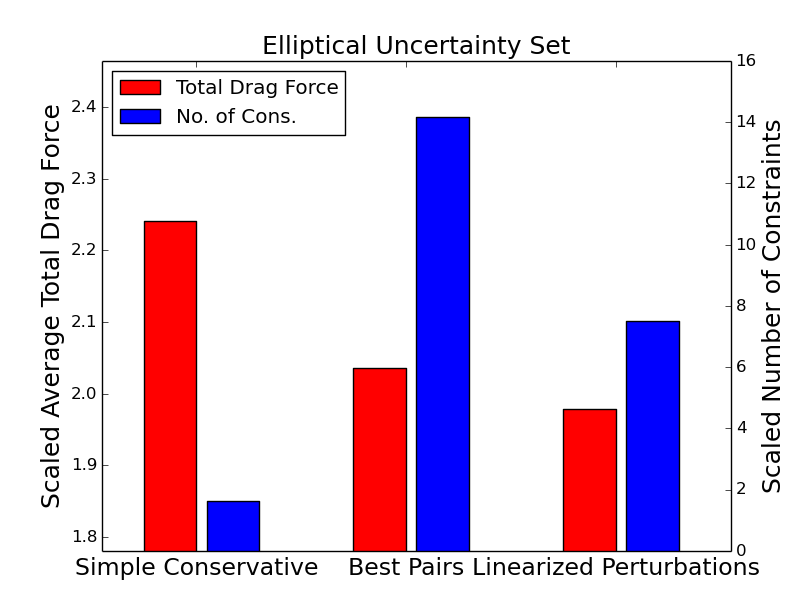
\includegraphics[height=2.3in]{signomial_simple_flight/ell.png}
        % \caption{Elliptical Uncertainty Set Objective Value}
    \end{subfigure}%
    ~ 
    \begin{subfigure}{0.49\textwidth}
        \centering
        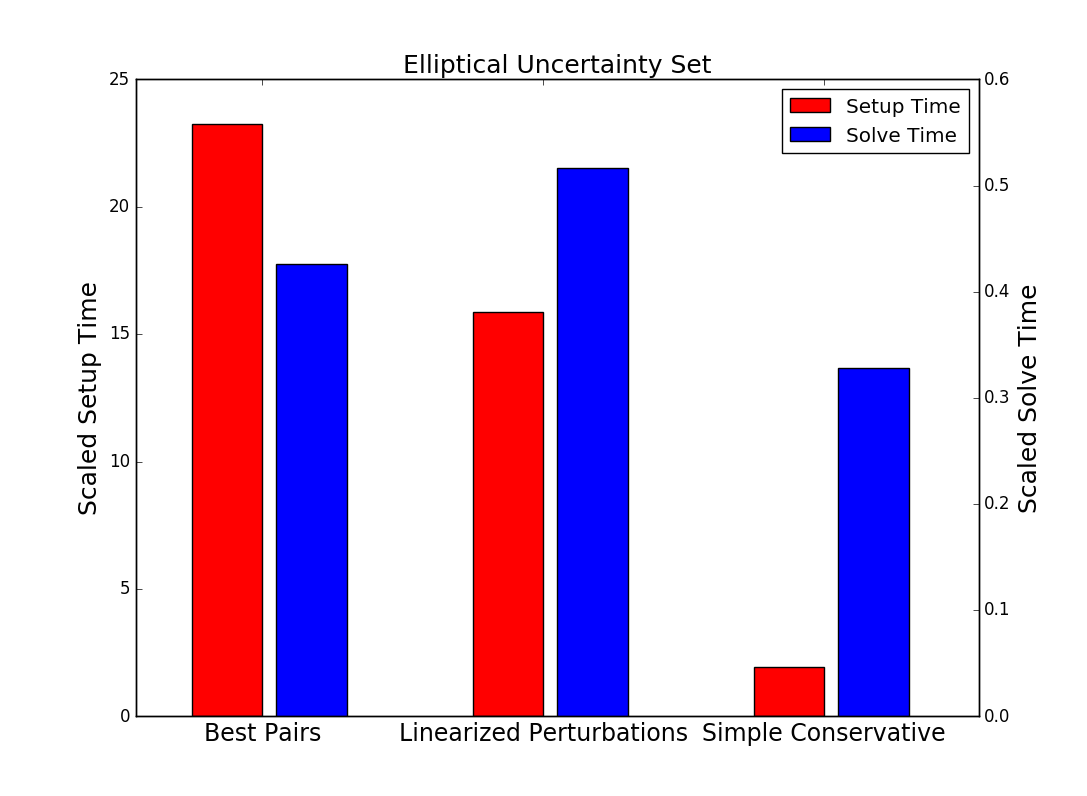
\includegraphics[height=2.3in]{signomial_simple_flight/ell_times.png}
        % \caption{Elliptical Uncertainty Set Probability of Failure}
    \end{subfigure}
    \caption{Robust signomial simple aircraft design results relative to the deterministic design problem.}
    \label{compare_signomial}
\end{figure}

\subsection{The Effect of Robustness}


%\textbf{TODO: update with 7-objective spider plots. First cite SP_tasopt, then show table and spider plots.
%Then show how robust results change the spider plots.}


One of the benefits of convex and difference-of-convex optimization methods is the ability to optimize for
different objectives~\cite{York2018}. For the aircraft model in question, we optimized for 7 different objectives, and show
the non-dimensionalized results in Table~\ref{tab:nondimresults}.

\begin{table}
    \resizebox{\textwidth}{!}{
    \csvautobooktabularcenter{figures/objective_table.csv}
    }
\caption{Non-dimensionalized variations in objective values with respect to the aircraft optimized
for different objectives. Objective values were normalized by the total fuel solution.}
    \label{tab:nondimresults}
\end{table}

To further demonstrate the capabilities of robust SPs in aircraft design,
we performed the optimization of the aircraft with no uncertainty and ellipsoidal uncertainty ($\Gamma = 1$)
for two more objective functions, and plotted the results on spider plots.
Spider plots are useful because they allow engineers to see the performance of different designs in a multi-objective
environment. Due to the large disparities in the potential values of design variables depending
on objective as shown in Table~\ref{tab:nondimresults}, we chose to demonstrate this using four objective functions
that would be expected to have a high degree of correlation and therefore yield similar aircraft designs. These were
 total (time and fuel) cost, total fuel, takeoff weight and mid-cruise lift-over-drag (L/D).

\begin{figure}
    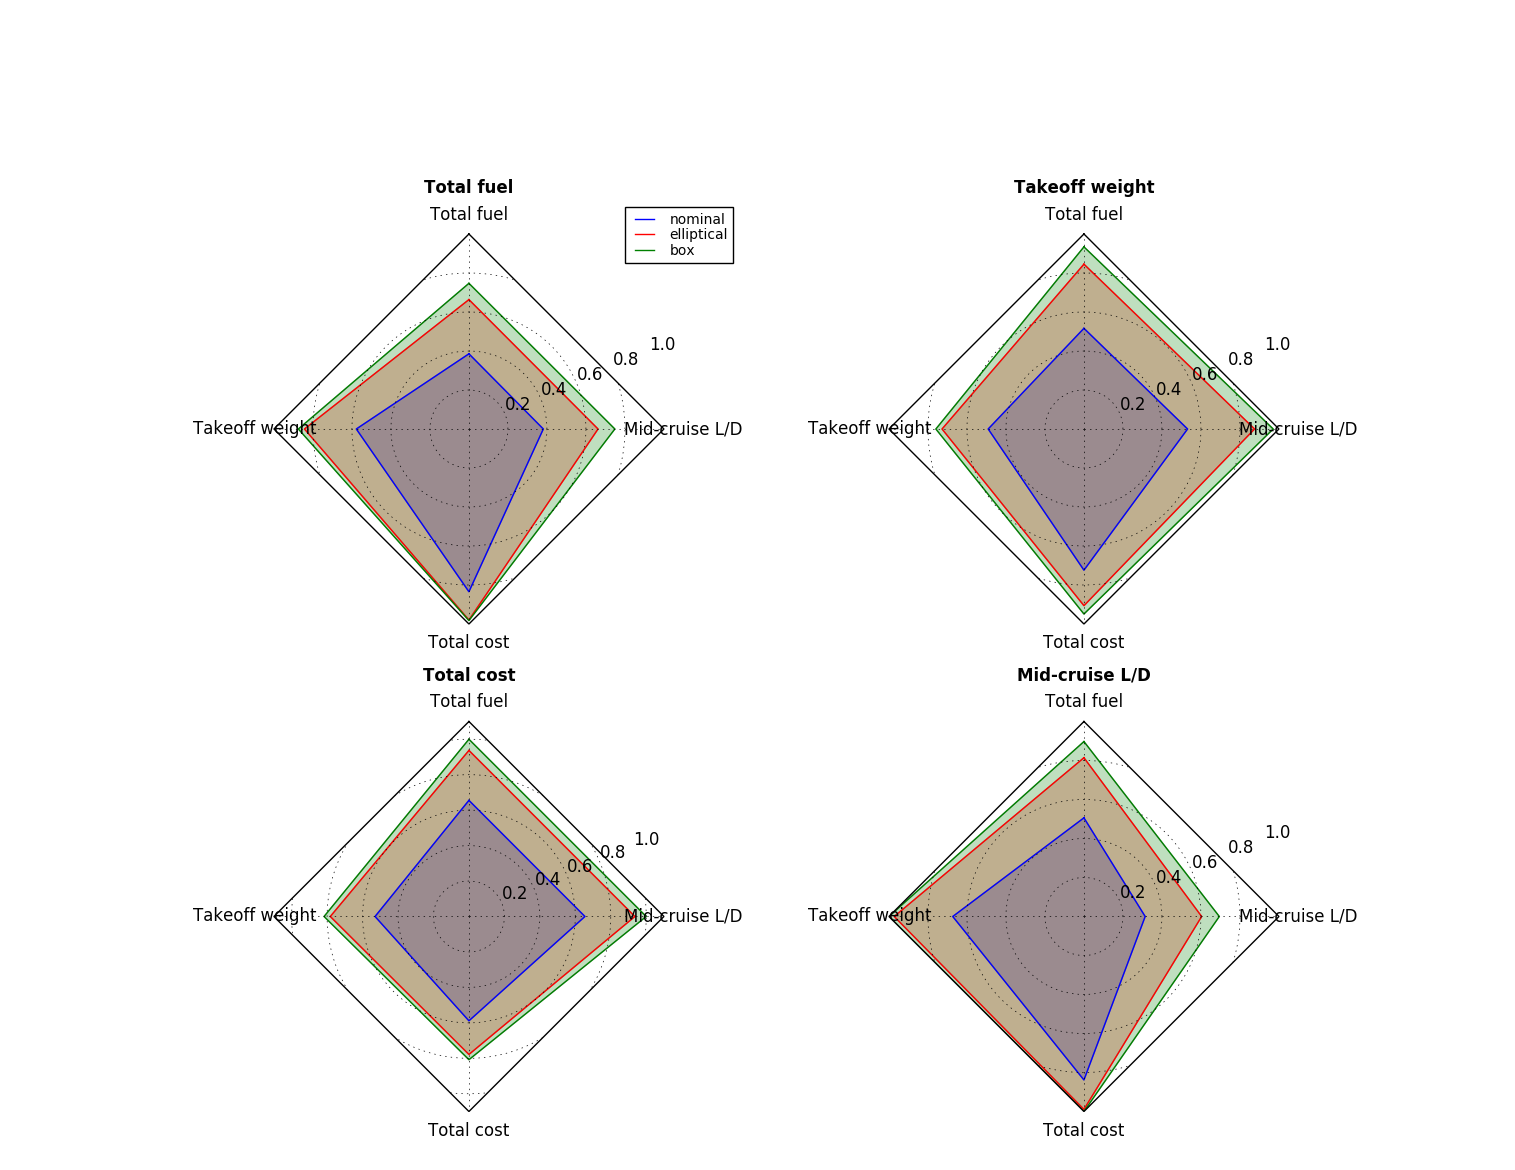
\includegraphics[width = 0.95\linewidth]{figures/4objradar.png}
    \caption{The spider plots of aircraft optimized for different objectives.
    The bolded titles are the design objectives for each plot, whereas the individual spiderwebs
    show the non-dimensionalized multiobjective performance of the aircraft designed under different
    uncertainty sets.}
    \label{fig:spider}
\end{figure}

In the spider plots in Figure~\ref{fig:spider}, it is possible to see the effect of robustness on
the different performance metrics of the different aircraft. One way to envision the multi-objective
performance of the aircraft is to consider the area contained within the web defined by the aircraft's
performance; the smaller the web area the beter.

For example, for the nominal case, which has no uncertainty, it is possible to see that
the aircraft designed for total fuel performs the best when all four objectives are considered.
However, this behavior changes when uncertainty is added. An aircraft optimized for total cost
(bottom left graph) with a box uncertainty set (in green) has better multiobjective performance
compared to an aircraft designed for total fuel with the same uncertainties.

This is an interesting result, because the presence of an uncertainty set is
shown to affect the efficacy of different objective functions to obtain solutions
with the best overall performance. If the three objective functions didn't
have high degree of coupling, that the internal areas of the solution triangles may differ
more significantly.

%\begin{figure}
%\begin{center}
%\begin{tikzpicture}[scale=0.5]
%\tkzKiviatDiagram{$\frac{W_f}{L/D}$,$D$,$W_f$}
%%solve for {W_f}{L/D}
%\tkzKiviatLine[thick,
%color=red,
%mark=ball,
%ball color=red,
%mark size=3pt,opacity=.2,
%fill=red!20](568.6/100,1051/150,13500/1500)
%%solve for D
%\tkzKiviatLine[thick,
%color=blue,
%mark=ball,
%mark size=3pt,
%fill=blue!20,
%opacity=.5](587/100,1024/150,13100/1500)
%% solve for {W_f}
%\tkzKiviatLine[thick,
%color=yellow,
%mark=ball,
%mark size=3pt,
%fill= yellow!20,
%opacity=.5](687.9/100,1155/150,11900/1500)
%\end{tikzpicture}
%\end{center}
%\caption[Uncertain Spider Plot]{Design optimization of the aircraft with ellipsoidal uncertainty for 3 different objective functions.
%The red, blue and yellow correspond to $\frac{W_f}{L/D}$, $D$, $W_f$ and objectives respectively.}
%% tkz-kiviat documentation here in FRENCH: http://mirror.jmu.edu/pub/CTAN/macros/latex/contrib/tkz/tkz-kiviat/doc/TKZdoc-kiviat-main.pdf
%\label{fig:spiderplotEllUncert}
%\end{figure}

\subsection{Goal Programming}

However, this assumes that we have an understanding of exactly how much risk we are
willing to tolerate. This begs the question, could we have risk as the output of our
model? This would suggest the following formulation:

\begin{align*}
    \text{maximize} &~\Gamma \\
    \text{s.t.}     &~f_i(x,u) \leq 0, i = 1,\ldots,n \\
                    & \norm{u} \leq \Gamma \\
                    &~f_0(x) \leq (1+\delta)f_0^*,~\delta \geq 0 \tag{a}
    \label{eq:goalprogramming}
\end{align*}

where $f_0^*$ is the optimum of the original problem in Formulation~\ref{eq:normform}, $\delta$
is a fractional measure of the objective that we are willing to sacrifice for robustness, which
gives $(1+\delta)f_0^*$ as the upper bound on the objective value.

We can also expand this framework to perform multivariate goal programming,
by changing (a) in the formulation~\ref{eq:goalprogramming} to include all
objectives we are interested in.

\begin{align*}
    f_{0,j}(x) \leq (1+\delta_j) f^*_{0,j},~\delta_j \geq 0,~i = 1,\ldots, m
    \label{eq:multigoal}
\end{align*}

The benefit of goal programming is that it allows us to explore multidisciplinary tradeoffs without
having to enumerate the design space along each objective direction. Furthermore, in design it is not obvious whether
an objective should in fact be a constraint instead. For example, it's not clear that the design
of an aircraft is useful if it consumes

\subsubsection{Changes in flight envelope}
